\section{Convolutional Neural Networks}

\subsection{Il primo problema con le immagini}
Le reti neurali convoluzionali vengono utilizzate e sono diventate famose per
l'elaborazione di immagini. Quando parliamo di \textit{fully connected
    networks} parliamo di reti dove ogni neurone è connesso con tutti i neuroni del
layer successivo. Questo significa che se abbiamo un'immagine di
\textbf{100x100 pixel}, avremo \textbf{10000 neuroni} nel layer di input.

\begin{equation}
    \sum_{i=1}^{k} d_h \cdot d_{h-1}
\end{equation}
per una rete con \textit{k} layer e dimensioni \textit{d} per ogni layer \textit{h}.

Questo numero di parametri è \textit{eccessivamente elevato}. Il numero di
connessioni raggiungerebbe un magnitudo altissimo contando le connessioni con i
layer successivi.

\subsection{Il secondo problema}
Spatial pattern e spatial hierarchies. (Da finire non ho capito).

\subsection{Come fa la rete a riconoscere i pattern}

La rete per riconoscere le immagini non può analizzare in totale l'immagine,
sarebbe eccessivamente costoso per i motivi precedenti.

\textbf{L'intuizione:} riconoscere pattern all'interno dell'immagine di \textbf{dimensioni ridotte}. Quando intendiamo
dimensioni ridotte, intendiamo anche \textbf{3x3} pixels. Questo è il motivo per cui le reti convoluzionali
sono chiamate \textbf{convoluzionali}: perché utilizzano la convoluzione per riconoscere i pattern.

L'algoritmo ad alto livello è il seguente:
\begin{enumerate}
    \item Prendere un'immagine
    \item Analizzare piccole porzioni dell'immagine
    \item Costruire elementi dell'immagine trovando elementi che si ripetono (pattern)
    \item Astrarre i pattern combinandoli tra loro
    \item Riconoscere l'immagine
\end{enumerate}

La nozione di \textbf{astrazione} e \textbf{connessione spaziale} è
fondamentale ed è l'intuizione dietro le reti convoluzionali.

\subsection{Convoluzione}

Parliamo dell'idea dietro la convoluzione. Partiamo dagli elementi
fondamentali.

\begin{itemize}
    \item Immagine in scala di grigiù
    \item Matrice di convoluzione \textbf{(kernel)}: Gli elementi all'interno della
          matrice sono \textbf{parametri}
\end{itemize}

%crea una matrice 10x10 di pixels in scala di grigi
\begin{figure}[H]
    \begin{center}

        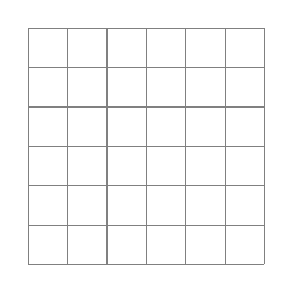
\begin{tikzpicture}
            \draw[step=0.5cm,color=gray] (0,0) grid (3,3);
        \end{tikzpicture}

    \end{center}
\end{figure}
\textbf{Nota:} nelle reti neurali convoluzionali non citiamo mai i neuroni.

\textbf{Obiettivo:} Creare una nuova immagine.

Ma come si applica? Come funziona la convoluzione?

Dobbiamo effettuare una moltiplicazione tra una sotto-matrice dell'immagine
principale e la matrice di convoluzoine (cioè il kernel). Ciò che ne viene
fuori è un \textbf{unico punto}.

\begin{figure}[H]
    \centering
    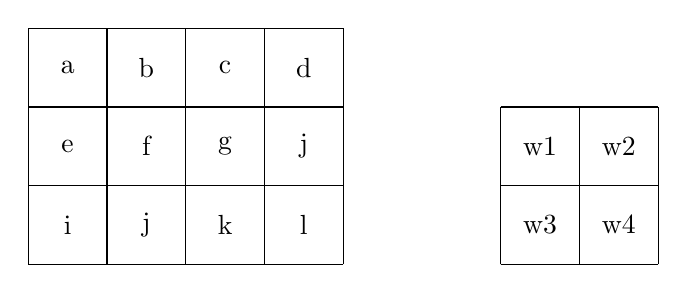
\begin{tikzpicture}
        % Prima matrice
        \draw (0,0) grid (4,3);
        \node at (0.5,2.5) {a};
        \node at (1.5,2.5) {b};
        \node at (2.5,2.5) {c};
        \node at (3.5,2.5) {d};
        \node at (0.5,1.5) {e};
        \node at (1.5,1.5) {f};
        \node at (2.5,1.5) {g};
        \node at (3.5,1.5) {j};
        \node at (0.5,0.5) {i};
        \node at (1.5,0.5) {j};
        \node at (2.5,0.5) {k};
        \node at (3.5,0.5) {l};

        % Seconda matrice
        \draw (6,0) grid (8,2);
        \node at (6.5,1.5) {w1};
        \node at (7.5,1.5) {w2};
        \node at (6.5,0.5) {w3};
        \node at (7.5,0.5) {w4};
    \end{tikzpicture}
\end{figure}

Per calcolare il primo punto con la convoluzione avremmo:
\begin{equation}
    aw_1 + bw_2 + ew_3 fw_4
\end{equation}

Questo per ogni \textbf{shift} del kernel nella matrice dell'immagine, andando
a calcolare i prossimi elementi:
\begin{equation}
    bw_1 + cw_2 + fw_3 + gw_4
\end{equation}

E continuando.

\textbf{Qual è il numero di parametri?}

\textbf{Nota:} Se nella feature map \textbf{troviamo un pattern}, ad esempio un quadrato 2x2, allora \textbf{sicuramente} questo sarà anche un \textbf{pattern più grande nella matrice principale},
poiché

\subsection{Padding}

Il "Padding" è una tecnica utilizzata nell'ambito del Machine Learning, in
particolare nell'elaborazione delle immagini. Quando si applica una
convoluzione utilizzando una "feature map" 3x3 a un'immagine, essa tende a
restringersi di 2 pixel lungo ciascuna dimensione. Questo può comportare la
perdita di informazioni ai bordi dell'immagine.

Per evitare questo effetto di restringimento, è possibile utilizzare il
"padding". Il padding consiste nell'aggiungere una cornice esterna all'immagine
con una larghezza e un'altezza adeguate. In altre parole, si aggiungono pixel
extra intorno all'immagine prima di eseguire la convoluzione.

L'obiettivo del padding è preservare le dimensioni originali dell'immagine
durante la convoluzione, consentendo così di mantenere tutte le informazioni
presenti ai bordi. Questo è particolarmente importante in applicazioni di
Machine Learning che coinvolgono il rilevamento di bordi, oggetti o
caratteristiche chiave nelle immagini.

\subsection{Strides}

Il concetto di \textbf{stride} nelle reti neurali convoluzionali (CNN) è
fondamentale per comprendere come i filtri scorrono attraverso i dati di input.
Il \textit{stride} rappresenta la distanza tra le posizioni in cui il filtro
viene applicato. Un \textbf{stride} maggiore porta a una riduzione della
dimensione dell'output, poiché il filtro salta più spazio alla volta. D'altro
canto, uno \textit{stride} minore comporta una maggiore sovrapposizione tra le
regioni in cui il filtro viene applicato, mantenendo una dimensione di output
più grande.

Comunque \textbf{riduci il numero di feature maps}.

\textbf{Nota generale}: Si possono usare diversi \textbf{kernels} e ogni kernel darà come risultato una \textbf{nuova feature map}.

\subsection{Esempio 1}

Immaginiamo di avere un input $32 \times 32$ come immagine.

\begin{itemize}
    \item Si usano 6 kernel
    \item Danno come risultato 6 feature maps 28x28
    \item Si sono persi 4 pixels sia in altezza che larghezza
    \item Il kernel era 5x5
    \item Il numero di parametri era $6 \cdot (5x5)$
\end{itemize}

Dopo questo si utilizza una tecnica che si chiama Pooling

\subsection{Pooling}

Il "Pooling" è una tecnica ampiamente utilizzata nell'ambito dell'apprendimento
automatico, specialmente nell'elaborazione delle immagini. Il suo obiettivo
principale è ridurre la dimensione dei dati mantenendo le caratteristiche più
importanti.

Il Pooling è un'operazione che riduce la dimensione di una rappresentazione
mantenendo le caratteristiche più rilevanti. Questo processo è spesso
utilizzato dopo la fase di convoluzione in una rete neurale convoluzionale
(CNN).

\subsubsection{Max Pooling}
Il Max Pooling suddivide una regione in celle e restituisce il valore massimo
all'interno di ciascuna cella. Questo aiuta a conservare le caratteristiche più
rilevanti, come i bordi o le texture.

Il Pooling ha diversi vantaggi:

\begin{itemize}
    \item Riduzione della dimensione dei dati, consentendo un addestramento più veloce.
    \item Riduzione del rischio di overfitting, poiché si mantengono solo le
          caratteristiche più importanti.
    \item Maggiore invarianza spaziale, poiché il Pooling considera la presenza delle
          caratteristiche, indipendentemente dalla loro posizione esatta nell'immagine.
\end{itemize}

Il Pooling è una tappa fondamentale in molte architetture di reti neurali
convoluzionali. Viene utilizzato per creare rappresentazioni più compatte e
significative dei dati, consentendo alle reti neurali di apprendere con
successo le caratteristiche più importanti delle immagini o dei dati in
ingresso.

\begin{itemize}
    \item Si applica il pooling sulle feature map di prima con una matrice $2 \times 2$
    \item Si passa da $28 \times 28$ a $14 \times 14$
\end{itemize}

E si ripete il processo di applicare la convoluzione sulle 6 feature map $14
    \times 14$, portano ad avere 16 feature map $10 \times 10$. Si riapplica ancora
il pooling e si avranno 16 feature map $5 \times 5$.

Alla fine si unisce tutto quanto insieme e si ha una \textbf{rete neurale
    standard}.

%insert picture
\begin{figure}[H]
    \begin{center}
        \includegraphics[scale=0.5]{images/conv.png}
        \caption{Esempio di rete neurale convoluzionale}
    \end{center}
\end{figure}

\subsection{Multiclass Classification Example}

\begin{lstlisting}[language=Python]
import tensorflow as tf
from tensorflow.keras import datasets, layers, models, optimizers
# CIFAR_10 is a set of 60K images 32x32 pixels on 3 channels
IMG_CHANNELS = 3
IMG_ROWS = 32
IMG_COLS = 32
#constant
BATCH_SIZE = 128
EPOCHS = 20
CLASSES = 10
VALIDATION_SPLIT = 0.2
OPTIM = tf.keras.optimizers.RMSprop()

#define the convnet
def build(input_shape, classes):
    model = models.Sequential()

    #32 e' il numero di kernel, 3x3 e' la grandezza del kernel
    model.add(layers.Convolution2D(32, (3, 3), activation='relu'
    , padding='valid', input_shape=input_shape))

    model.add(layers.MaxPooling2D(pool_size=(2, 2)))
    model.add(layers.Dropout(0.25))

    #Flatten e' necessario per passare da 3D a 1D (Diventa un vettore)
    model.add(layers.Flatten())

    #Qui diventa una rete neurale standard
    model.add(layers.Dense(512, activation='relu'))
    model.add(layers.Dropout(0.5))

    #Qui abbiamo tanti nodi di output quante sono le classi del dataset
    model.add(layers.Dense(classes, activation='softmax'))
    return model

# data: shuffled and split between train and test sets
(X_train, y_train), (X_test, y_test) = datasets.cifar10.load_data()
# normalize
X_train, X_test = X_train / 255.0, X_test / 255.0
# convert to categorical
# convert class vectors to binary class matrices
y_train = tf.keras.utils.to_categorical(y_train, CLASSES)
y_test = tf.keras.utils.to_categorical(y_test, CLASSES)
model=build((IMG_ROWS, IMG_COLS, IMG_CHANNELS), CLASSES)
model.summary()

# use TensorBoard,
callbacks = [
    # Write TensorBoard logs to `./logs` directory
    tf.keras.callbacks.TensorBoard(log_dir='./logs')
]
# train
model.compile(loss='categorical_crossentropy', optimizer=OPTIM, metrics=['accuracy'])

model.fit(X_train, y_train, batch_size=BATCH_SIZE, epochs=EPOCHS, 
validation_split=VALIDATION_SPLIT, verbose=VERBOSE, callbacks=callbacks)

score = model.evaluate(X_test, y_test,
batch_size=BATCH_SIZE, verbose=VERBOSE)
print("\nTest score:", score[0])
print('Test accuracy:', score[1])

\end{lstlisting}

\subsection{Nozioni alla lavagna}
\textbf{Quante immagini ci servono per trainare una NN?}

Prendiamo il concetto di posizione dell'oggetto nell'immagine, se volessimo
parlare di \textit{object recognition}. Le reti neurali dovrebbero essere
\textit{immuni} al concetto di traslazione. La posizione, quindi, non dovrebbe
influire molto sul risultato finale. Per quanto riguarda \textbf{la scala}
dell'oggetto, qui è diverso. Conviene avere diverse immagini dello stesso
oggetto con dimensioni diverse, poiché, in questo caso, influirebbe sul
risultato finale della classificazione. Anche per quanto riguarda la
\textbf{rotazione}, si ha lo stesso discorso della scala. Anche in quest caso
conviene avere più immagini dello stesso oggetto con \textbf{rotazioni
    diverse}.

\begin{quote}
    Per ogni immagine, inserire altre immagini con scala e rotazione diversa dell'oggetto.
\end{quote}

\textbf{Esempio del mondo reale:} I segnali stadali di velocità. 
Per poterli riconoscere c'è la necessità di avere diverse immagini 
a divers a distanza per avere un allenamento corretto della rete.

\newpage